\section{Optimization}%
\label{sec:optimization}

\subsection{Gradient Descent}%
\label{sub:gradient_descent}
Gradient descent is an iterative optimization algorithm, utilizing the first derivative of the loss function $L$ with respect to all function parameters $\theta$. To recall, a single iteration of gradient descent is as follows:
\begin{align}
         \theta'=\theta-\alpha \frac{\delta}{\delta \theta}L(\theta)
\end{align}
$\alpha$ is the \emph{learning rate}, an arbitrary positive scaling factor, determining the magnitude of the update \wrt{} the gradient.

\begin{figure}[htpb]
        \centering
        % This file was created by tikzplotlib v0.9.1.
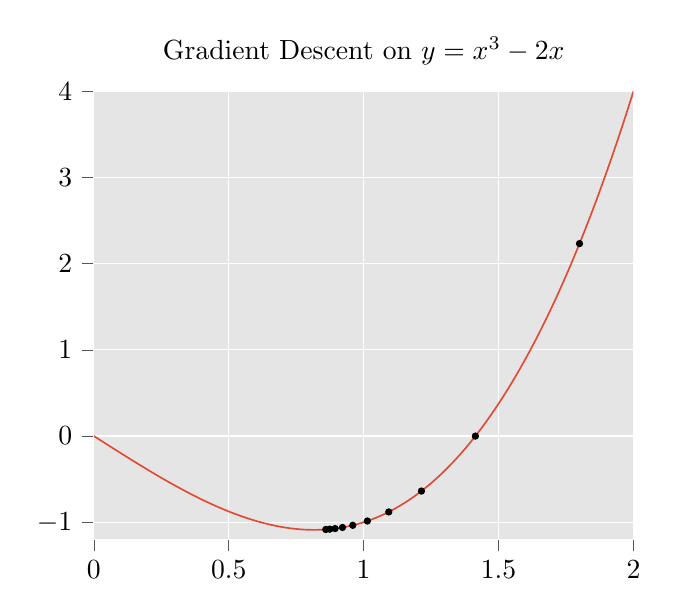
\begin{tikzpicture}

\definecolor{color0}{rgb}{0.886274509803922,0.290196078431373,0.2}

\begin{axis}[
axis background/.style={fill=white!89.8039215686275!black},
axis line style={white},
tick align=outside,
tick pos=left,
title={Gradient Descent on $y=x^3-2x$},
x grid style={white},
xmajorgrids,
xmin=0, xmax=2,
xtick style={color=white!33.3333333333333!black},
y grid style={white},
ymajorgrids,
ymin=-1.2, ymax=4,
ytick style={color=white!33.3333333333333!black}
]
\addplot [semithick, color0]
table {%
0 0
0.0202020201832056 -0.0403957962989807
0.0404040403664112 -0.0807421207427979
0.060606062412262 -0.120989516377449
0.0808080807328224 -0.161088496446609
0.101010099053383 -0.200989589095116
0.121212124824524 -0.240643352270126
0.141414135694504 -0.280000269412994
0.161616161465645 -0.319010943174362
0.181818187236786 -0.357625842094421
0.202020198106766 -0.395795524120331
0.222222223877907 -0.433470517396927
0.242424249649048 -0.470601350069046
0.262626260519028 -0.50713849067688
0.282828271389008 -0.543032586574554
0.30303031206131 -0.578234136104584
0.32323232293129 -0.612693607807159
0.34343433380127 -0.646361589431763
0.363636374473572 -0.67918860912323
0.383838385343552 -0.711125135421753
0.404040396213531 -0.742121756076813
0.424242436885834 -0.772128999233246
0.444444447755814 -0.801097393035889
0.464646458625793 -0.828977465629578
0.484848499298096 -0.855719745159149
0.505050480365753 -0.881274700164795
0.525252521038055 -0.905593037605286
0.545454561710358 -0.928625106811523
0.565656542778015 -0.950321435928345
0.585858583450317 -0.970632791519165
0.60606062412262 -0.989509463310242
0.626262605190277 -1.00690197944641
0.646464645862579 -1.0227609872818
0.666666686534882 -1.03703701496124
0.686868667602539 -1.04968059062958
0.707070708274841 -1.06064212322235
0.727272748947144 -1.06987226009369
0.747474730014801 -1.07732152938843
0.767676770687103 -1.08294034004211
0.787878811359406 -1.08667945861816
0.808080792427063 -1.08848929405212
0.828282833099365 -1.08832025527954
0.848484873771667 -1.08612298965454
0.868686854839325 -1.08184790611267
0.888888895511627 -1.07544589042664
0.909090936183929 -1.06686699390411
0.929292917251587 -1.05606210231781
0.949494957923889 -1.04298162460327
0.969696998596191 -1.02757596969604
0.989898979663849 -1.00979590415955
1.01010096073151 -0.989591956138611
1.03030300140381 -0.966914415359497
1.05050504207611 -0.941713929176331
1.07070708274841 -0.913940906524658
1.09090912342072 -0.883546233177185
1.11111116409302 -0.850480079650879
1.13131308555603 -0.814693212509155
1.15151512622833 -0.776136040687561
1.17171716690063 -0.734759092330933
1.19191920757294 -0.690512895584106
1.21212124824524 -0.643347978591919
1.23232328891754 -0.593214869499207
1.25252521038055 -0.540064573287964
1.27272725105286 -0.48384690284729
1.29292929172516 -0.424512386322021
1.31313133239746 -0.362012147903442
1.33333337306976 -0.296296119689941
1.35353529453278 -0.227315664291382
1.37373733520508 -0.155020475387573
1.39393937587738 -0.0793612003326416
1.41414141654968 -0.000288724899291992
1.43434345722198 0.0822467803955078
1.45454549789429 0.168294668197632
1.4747474193573 0.257903814315796
1.4949494600296 0.35112452507019
1.5151515007019 0.448006153106689
1.53535354137421 0.548598051071167
1.55555558204651 0.652949333190918
1.57575762271881 0.761110067367554
1.59595954418182 0.873128652572632
1.61616158485413 0.989055633544922
1.63636362552643 1.10894083976746
1.65656566619873 1.23283243179321
1.67676770687103 1.3607804775238
1.69696974754333 1.49283504486084
1.71717166900635 1.62904405593872
1.73737370967865 1.76945853233337
1.75757575035095 1.91412734985352
1.77777779102325 2.0631000995636
1.79797983169556 2.21642637252808
1.81818187236786 2.37415528297424
1.83838379383087 2.53633522987366
1.85858583450317 2.70301818847656
1.87878787517548 2.87425208091736
1.89898991584778 3.05008697509766
1.91919195652008 3.23057150840759
1.93939399719238 3.41575574874878
1.9595959186554 3.60568809509277
1.9797979593277 3.80042004585266
2 4
};
\addplot [semithick, black, mark=*, mark size=1, mark options={solid}, only marks]
table {%
1.79999995231628 2.23199939727783
1.41400003433228 -0.000854015350341797
1.21409058570862 -0.63859224319458
1.09298825263977 -0.880267262458801
1.01379477977753 -0.985631704330444
0.95962780714035 -1.03554821014404
0.921494960784912 -1.06049966812134
0.894122004508972 -1.07343447208405
0.874203860759735 -1.08031272888184
0.859569013118744 -1.08403778076172
};
\end{axis}

\end{tikzpicture}

        \caption{Demonstration of gradient descent convergence: 10 iterations with $\alpha =5\times 10^{-2}$ and $\theta_0=1.8$.}
        \label{fig:gradient_demo}
\end{figure}

\autoref{fig:gradient_demo} is a toy example of gradient descent, but it generalizes to more complicated problems such as Reversing Nearness.

\subsubsection{Partial Derivative of Loss Function}%
\label{ssub:derivative_of_loss_function}
A partial derivative is the derivative of a multi-variable function \wrt{} a single variable, and is denoted by $\frac{\delta}{\delta x}$ instead of $\frac{d}{dx}$. Hence, our goal is to find the Jacobian matrix $\bm{J}$ of $L(S)$ \wrt{} $S$, defined as follows:
 \begin{align}
     \bm{J}=\frac{\delta L(S)}{\delta S}= \begin{bmatrix}
                 \frac{\delta L(S)}{\delta S_{1,1}}&\cdots &\frac{\delta L(S)}{\delta S_{1,N^2}}\\
                 \vdots &\ddots &\vdots \\
                 \frac{\delta L(S)}{\delta S_{N^2,1}}&\cdots &\frac{\delta L(S)}{\delta S_{N^2,N^2}}\\
         \end{bmatrix}
         \label{eq:jacobian_definition}
\end{align}

To do that, a general solution to the partial derivative: $ \frac{\delta L(S)}{\delta S_{i,j}}$, is required. Recall that the loss function is defined as
\begin{align}
    L(S)=\frac{1}{2}\sum_{a}^{N^2} \sum_{b}^{N^2} \sum_{c}^{N^2} \sum_{d}^{N^2} S_{a,b} S_{c,d} C(O)_{a,c}C(O)_{b,d}-c
\end{align}
When evaluating $\bm{J}_{i,j}$, only $S_{i,j}$ is treated as a variable, whereas others are treated as constants, evaluating to $0$ after differentiation. Note that $S_{i,j}$ is only included within the loss when $(a,b)=(i,j)$ or $(c,d)=(i,j)$ or both. The derivatives of the terms of for the respective cases are as follows:
\begin{align}
    \bm{A}=\frac{\delta L(S)}{\delta S_{i,j}}&=\frac{\delta}{\delta S_{i,j}}\left(\frac{1}{2}\sum_{c}^{N^2} \sum_{d}^{N^2} S_{\highlight{i,j}} S_{c,d} C(O)_{\highlight{i},c}C(O)_{\highlight{j},d}\right)&\text{first case}\nonumber\\
              &=\frac{1}{2}\sum_{c}^{N^2} \sum_{d}^{N^2} S_{c,d} C(O)_{i,c}C(O)_{j,d}&\nonumber\\
    \bm{B}=\frac{\delta L(S)}{\delta S_{i,j}}&=\frac{\delta}{\delta S_{i,j}}\left(\frac{1}{2}\sum_{a}^{N^2} \sum_{b}^{N^2} S_{a,b} S_{\highlight{i,j}} C(O)_{a,\highlight{i}}C(O)_{b,\highlight{j}}\right)&\text{second case}\nonumber\\
              &=\frac{1}{2}\sum_{a}^{N^2} \sum_{b}^{N^2} S_{a,b} C(O)_{a,i}C(O)_{b,j}&\nonumber\\
    \bm{C}=\frac{\delta L(S)}{\delta S_{i,j}}&=\frac{\delta}{\delta S_{i,j}}\left(\frac{1}{2}S_{\highlight{i,j}} S_{\highlight{i,j}} C(O)_{\highlight{i,i}}C(O)_{\highlight{j,j}}\right)&\text{third case}\nonumber\\
              &=S_{i,j} C(O)_{i,i}C(O)_{j,j}&\nonumber\\
              &=0&
\end{align}
$\bm{C}$ is $0$ due because it includes the distance of a token against itself. Therefore, $\frac{\delta L(S)}{\delta S_{i,j}}$, taking into account all 3 cases, is equal to $\bm{A}+\bm{B}-\bm{C}=\bm{A}+\bm{B}$, but it can be simplified,
\begin{align}
    \frac{\delta L(S)}{\delta S_{i,j}}&=\bm{A}+\bm{B}\nonumber\\
    &=\frac{1}{2}\left(\sum_{c}^{N^2} \sum_{d}^{N^2} S_{c,d} C(O)_{i,c}C(O)_{j,d}+\sum_{a}^{N^2} \sum_{b}^{N^2} S_{a,b} C(O)_{a,i}C(O)_{b,j}\right)\nonumber\\
    &=\frac{1}{2}\left(\sum_{\highlight{a}}^{N^2} \sum_{\highlight{b}}^{N^2} S_{\highlight{a,b}} C(O)_{i,\highlight{a}}C(O)_{j,\highlight{b}}+\sum_{a}^{N^2} \sum_{b}^{N^2} S_{a,b} C(O)_{a,i}C(O)_{b,j}\right)\label{eq:simplification_1}\\
    &=\frac{1}{2}\left(\sum_{a}^{N^2} \sum_{b}^{N^2} S_{a,b} C(O)_{\highlight{a,i}}C(O)_{j,b}+\sum_{a}^{N^2} \sum_{b}^{N^2} S_{a,b} C(O)_{a,i}C(O)_{\highlight{j,b}}\right)\label{eq:simplification_2}\\
    &=\sum_{a}^{N^2} \sum_{b}^{N^2} S_{a,b} C(O)_{a,i}C(O)_{j,b}
\end{align}
\autoref{eq:simplification_1} utilizes the independence of the 2 summations, equating the summation variables. \autoref{eq:simplification_2} utilizes the symmetric nature of $C(O)$, in order to have $a$ and $b$ along the same axes within all terms.

For example, $\frac{\delta L(S)}{\delta S_{2,3}}$ for \autoref{fig:superpositionShade} is calculated as follows,
\begin{align}
    \frac{\delta L(S)}{\delta S_{1,1}}&=\sum_{a}^{N^2} \sum_{b}^{N^2} S_{a,b} C(O)_{a,i}C(O)_{j,b}\nonumber\\
      &=\sum_{a}^{N^2} \sum_{b}^{N^2}
      \begin{bmatrix}
          1&0&0&0\\
          0&1&0&0\\
          0&0&0&1\\
          0&0&1&0
      \end{bmatrix}\odot
      \begin{bmatrix}
          1&1&1&1\\
          0&0&0&0\\
          2&2&2&2\\
          1&1&1&1
      \end{bmatrix}\odot
      \begin{bmatrix}
          1&2&0&1\\
          1&2&0&1\\
          1&2&0&1\\
          1&2&0&1
      \end{bmatrix}\label{eq:partial_example}\\
      &=\sum_{a}^{N^2} \sum_{b}^{N^2}
      \begin{bmatrix}
          1&0&0&0\\
          0&0&0&0\\
          0&0&0&2\\
          0&0&0&0
      \end{bmatrix}\nonumber\\
      &=3
\end{align}
$C(O)_{a,i}$ and $C(O)_{j,b}$ within \autoref{eq:partial_example} are repeated along the columns and rows respectively, due to $i$ and $j$ being constant \wrt{} $a$ and $b$ respectively. Computing $\bm{J}$ for \autoref{fig:superpositionShade} results in,
\begin{align}
    \bm{J}=\begin{bmatrix}
          5&5&3&3\\
          5&5&3&3\\
          3&3&5&5\\
          3&3&5&5
      \end{bmatrix}
    \label{eq:jacobian_example}
\end{align}

Now, a naive approach would be to apply gradient descent as follows:
\begin{align}
    S'=S-\alpha\bm{J}
    \label{eq:naive_descent}
\end{align}
But doing so would not take into the constraints involved within discrete optimization (that generalize to continuous optimization).

\subsection{Generalization of Discrete Constraints}%
\label{sub:constraints}

\subsubsection{Doubly Stochastic Matrices}%
\label{ssub:doubly_stochastic_matrices}
First of all, \emph{negative weights are nonsensical}, since weights should reflect the portion of the token located within a certain position.

In the discrete problem, within $X$ or $O$, every position has a \emph{single} unique token, and every token has a \emph{single} unique position. Generalizing this to superposition, note that all rows and columns should sum to 1 (e.g., \autoref{fig:superpositionShade}). Intuitively, a superposition grid divides the weight of each token value, into fragments whose weights sum to 1, with every position containing in total weight 1, albeit from fragments and not \emph{whole} tokens.

Following from these observations, $S$ is said to be doubly stochastic. That is, any matrix $A$ with only non-negative values and
\begin{align}
    \sum_i A_{i,j}=\sum_j A_{i,j}=1
\end{align}
is doubly stochastic.\cite{weissteinDoubly} Therefore, to enforce this constraint, the superposition $S$ must remain doubly stochastic after the gradient descent update, or else, the weights could be set to 0, causing a loss of  $0-c$.

\subsubsection{Sinkhorn-Knopp Algorithm}%
\label{ssub:sinkhorn_knopp_algorithm}
This section explains the algorithm used within \autoref{ssub:zero_line_sum_modified_jacobian}.

A well-known algorithm to convert any non-negative matrix\footnote{\label{non-negative-caveat}having at least 1 positive value in each row and column} into a doubly stochastic matrix is the Sinkhorn-Knopp algorithm (also named RAS).\cite{sinkhorn1967concerning} There is a proof\cite{borobia1998matrix} and several papers analyzing its convergence.\cite{chakrabarty2018better,knight2008sinkhorn} Nonetheless, the algorithm itself is simple: alternating the normalization of rows and columns of a matrix. Here, ``normalization'' is defined as forming a sum of 1, by dividing each element within each row or column by the sum of the row or column.

Let $K$ be an $n\times n$ non-negative matrix.\footnote{see \autoref{non-negative-caveat}} A single iteration of RAS is defined as follows:
\begin{align}
        K'=&\begin{bmatrix}
                (\Sigma_j^N K_{1,j})^{-1}\\
                &\ddots{}\\
                &&(\Sigma_j^N K_{N,j})^{-1}
        \end{bmatrix}K &&\text{normalizing rows}\nonumber\\
            \ras(K)=K''=K'&\begin{bmatrix}
                (\Sigma_i^N K'_{i,1})^{-1}\\
                &\ddots{}\\
                &&(\Sigma_i^N K'_{i,N})^{-1}
        \end{bmatrix}&&\text{normalizing columns}
\end{align}
The scaling matrices are diagonal (non-diagonal elements are $0$s). Let $\ras^n(K)$ indicate $n$ iterations of RAS on $K$, i.e., $\ras^2(K)=\ras(\ras(K))$.

\autoref{fig:ras_demo} demonstrates the effectiveness of RAS in normalizing randomly sampled matrices. Graphed on the y-axis is the error: the squared distance between the sums of the rows and columns, and 1, defined as,
\begin{align}
        E(X)=\sum^N_i\left(\left(\sum^N_jX_{i,j}\right)-1\right)^2+\sum^N_j\left(\left(\sum^N_iX_{i,j}\right)-1\right)^2
\end{align}

\begin{figure}[htpb]
        \centering
        % This file was created by tikzplotlib v0.9.1.
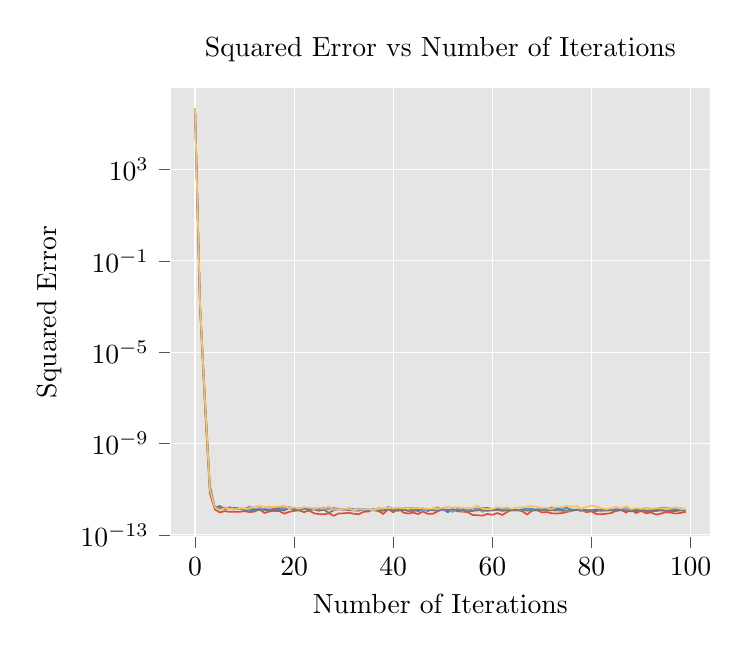
\begin{tikzpicture}

\definecolor{color0}{rgb}{0.886274509803922,0.290196078431373,0.2}
\definecolor{color1}{rgb}{0.203921568627451,0.541176470588235,0.741176470588235}
\definecolor{color2}{rgb}{0.596078431372549,0.556862745098039,0.835294117647059}
\definecolor{color3}{rgb}{0.984313725490196,0.756862745098039,0.368627450980392}

\begin{axis}[
axis background/.style={fill=white!89.8039215686275!black},
axis line style={white},
log basis y={10},
tick align=outside,
tick pos=left,
title={Squared Error vs Number of Iterations},
x grid style={white},
xlabel={Number of Iterations},
xmajorgrids,
xmin=-4.95, xmax=103.95,
xtick style={color=white!33.3333333333333!black},
y grid style={white},
ylabel={Squared Error},
ymajorgrids,
ymin=8.68476415176487e-14, ymax=3811887.27502007,
ymode=log,
ytick style={color=white!33.3333333333333!black}
]
\addplot [semithick, color0]
table {%
0 481023.09375
1 0.00103783328086138
2 4.61336888690767e-08
3 6.49791331852612e-12
4 1.31095134747738e-12
5 9.52127265918534e-13
6 1.09423581307055e-12
7 1.00541797110054e-12
8 1.02673425317334e-12
9 1.01252339845814e-12
10 1.07647224467655e-12
11 9.9120711638534e-13
12 1.03739239420975e-12
13 1.32516220219259e-12
14 9.05941988094128e-13
15 1.04805053524615e-12
16 1.11555209514336e-12
17 1.09778852674935e-12
18 8.41993141875719e-13
19 1.01607611213694e-12
20 1.10844666778576e-12
21 1.21502807814977e-12
22 9.80548975348938e-13
23 1.15818465928896e-12
24 8.77520278663724e-13
25 8.06466005087714e-13
26 7.85149723014911e-13
27 8.81072992342524e-13
28 6.78568312650896e-13
29 8.63309423948522e-13
30 8.73967564984923e-13
31 9.2370555648813e-13
32 8.38440428196918e-13
33 7.88702436693711e-13
34 1.01607611213694e-12
35 1.05160324892495e-12
36 1.30029320644098e-12
37 1.10489395410696e-12
38 8.20676859802916e-13
39 1.35358391162299e-12
40 9.62785406954936e-13
41 1.45661260830821e-12
42 9.52127265918534e-13
43 8.4909856923332e-13
44 9.41469124882133e-13
45 8.13571432445315e-13
46 1.04805053524615e-12
47 8.24229573481716e-13
48 8.31335000839317e-13
49 1.07291953099775e-12
50 1.33937305690779e-12
51 1.02673425317334e-12
52 1.31095134747738e-12
53 1.08357767203415e-12
54 1.03028696685215e-12
55 9.87654402706539e-13
56 7.42517158869305e-13
57 7.21200876796502e-13
58 6.89226453687297e-13
59 8.17124146124115e-13
60 7.49622586226906e-13
61 8.95283847057726e-13
62 7.38964445190504e-13
63 9.98312543742941e-13
64 1.26831878333178e-12
65 1.22213350550737e-12
66 1.08002495835535e-12
67 7.74491581978509e-13
68 1.13331566353736e-12
69 1.18660636871937e-12
70 9.55679979597335e-13
71 9.87654402706539e-13
72 8.73967564984923e-13
73 8.56203996590921e-13
74 8.91731133378926e-13
75 9.80548975348938e-13
76 1.16529008664656e-12
77 1.25766064229538e-12
78 1.17594822768297e-12
79 9.9120711638534e-13
80 1.05870867628255e-12
81 8.13571432445315e-13
82 7.92255150372512e-13
83 8.38440428196918e-13
84 8.88178419700125e-13
85 1.15107923193136e-12
86 1.21858079182857e-12
87 9.37916411203332e-13
88 1.29674049276218e-12
89 8.91731133378926e-13
90 1.11555209514336e-12
91 8.81072992342524e-13
92 9.48574552239734e-13
93 7.67386154620908e-13
94 8.4909856923332e-13
95 9.69890834312537e-13
96 9.41469124882133e-13
97 8.45545855554519e-13
98 9.09494701772928e-13
99 1.00186525742174e-12
};
\addplot [semithick, color1]
table {%
0 487870.4375
1 0.00108947034459561
2 5.42636904299343e-08
3 8.494538406012e-12
4 1.52766688188422e-12
5 1.48148160405981e-12
6 1.54187773659942e-12
7 1.4175327578414e-12
8 1.51345602716901e-12
9 1.48148160405981e-12
10 1.24700250125898e-12
11 1.23279164654377e-12
12 1.21858079182857e-12
13 1.4495071809506e-12
14 1.23989707390137e-12
15 1.28252963804698e-12
16 1.32871491587139e-12
17 1.18660636871937e-12
18 1.32160948851379e-12
19 1.4459544672718e-12
20 1.36779476633819e-12
21 1.4281908988778e-12
22 1.57740487338742e-12
23 1.25766064229538e-12
24 1.4281908988778e-12
25 1.34292577058659e-12
26 1.52056145452661e-12
27 1.4033219031262e-12
28 1.47082346302341e-12
29 1.31095134747738e-12
30 1.27542421068938e-12
31 1.4175327578414e-12
32 1.32160948851379e-12
33 1.19015908239817e-12
34 1.27897692436818e-12
35 1.20081722343457e-12
36 1.31805677483499e-12
37 1.14397380457376e-12
38 1.36424205265939e-12
39 1.26121335597418e-12
40 1.29674049276218e-12
41 1.13686837721616e-12
42 1.33937305690779e-12
43 1.11199938146456e-12
44 1.37845290737459e-12
45 1.06936681731895e-12
46 1.37134748001699e-12
47 1.08357767203415e-12
48 1.4317436125566e-12
49 1.17239551400417e-12
50 1.33937305690779e-12
51 9.73443547991337e-13
52 1.29318777908338e-12
53 1.07291953099775e-12
54 1.35358391162299e-12
55 1.11555209514336e-12
56 1.4459544672718e-12
57 1.33582034322899e-12
58 1.46016532198701e-12
59 1.50990331349021e-12
60 1.35713662530179e-12
61 1.35713662530179e-12
62 1.424638185199e-12
63 1.3997691894474e-12
64 1.31805677483499e-12
65 1.19371179607697e-12
66 1.28252963804698e-12
67 1.406874616805e-12
68 1.35358391162299e-12
69 1.25766064229538e-12
70 1.34647848426539e-12
71 1.35003119794419e-12
72 1.56319401867222e-12
73 1.3962164757686e-12
74 1.54543045027822e-12
75 1.49213974509621e-12
76 1.25055521493778e-12
77 1.27187149701058e-12
78 1.26831878333178e-12
79 1.21502807814977e-12
80 1.15107923193136e-12
81 1.06936681731895e-12
82 1.29318777908338e-12
83 1.32160948851379e-12
84 1.16529008664656e-12
85 1.12976294985856e-12
86 1.19015908239817e-12
87 1.14042109089496e-12
88 1.05870867628255e-12
89 1.09778852674935e-12
90 1.16173737296776e-12
91 1.10844666778576e-12
92 1.06936681731895e-12
93 1.10134124042816e-12
94 1.16173737296776e-12
95 1.10844666778576e-12
96 1.06936681731895e-12
97 1.10134124042816e-12
98 1.16173737296776e-12
99 1.10844666778576e-12
};
\addplot [semithick, color2]
table {%
0 483571.625
1 0.00135559169575572
2 9.83107923957505e-08
3 1.40119027491892e-11
4 1.68753899743024e-12
5 1.68753899743024e-12
6 1.27897692436818e-12
7 1.66267000167863e-12
8 1.34647848426539e-12
9 1.389111048411e-12
10 1.3962164757686e-12
11 1.74082970261225e-12
12 1.33582034322899e-12
13 1.47082346302341e-12
14 1.33582034322899e-12
15 1.72306613421824e-12
16 1.45661260830821e-12
17 1.55253587763582e-12
18 1.47082346302341e-12
19 1.65201186064223e-12
20 1.29674049276218e-12
21 1.31450406115619e-12
22 1.30384592011978e-12
23 1.49569245877501e-12
24 1.30739863379858e-12
25 1.33937305690779e-12
26 1.22568621918617e-12
27 1.36424205265939e-12
28 1.3962164757686e-12
29 1.4175327578414e-12
30 1.23279164654377e-12
31 1.424638185199e-12
32 1.15463194561016e-12
33 1.4139800441626e-12
34 1.23989707390137e-12
35 1.29674049276218e-12
36 1.16529008664656e-12
37 1.47082346302341e-12
38 1.35358391162299e-12
39 1.66977542903624e-12
40 1.389111048411e-12
41 1.53121959556302e-12
42 1.4459544672718e-12
43 1.51345602716901e-12
44 1.47437617670221e-12
45 1.48148160405981e-12
46 1.16173737296776e-12
47 1.30029320644098e-12
48 1.29674049276218e-12
49 1.60937929649663e-12
50 1.16529008664656e-12
51 1.29674049276218e-12
52 1.00541797110054e-12
53 1.4281908988778e-12
54 1.03739239420975e-12
55 1.29318777908338e-12
56 1.08713038571295e-12
57 1.4530598946294e-12
58 1.01252339845814e-12
59 1.27542421068938e-12
60 1.15107923193136e-12
61 1.21147536447097e-12
62 1.08357767203415e-12
63 1.18305365504057e-12
64 1.14397380457376e-12
65 1.14752651825256e-12
66 1.25055521493778e-12
67 1.30029320644098e-12
68 1.17950094136177e-12
69 1.33582034322899e-12
70 1.18305365504057e-12
71 1.21147536447097e-12
72 1.17594822768297e-12
73 1.16173737296776e-12
74 1.11199938146456e-12
75 1.04094510788855e-12
76 1.08002495835535e-12
77 1.23989707390137e-12
78 1.06226138996135e-12
79 1.14752651825256e-12
80 1.14042109089496e-12
81 1.31805677483499e-12
82 1.04805053524615e-12
83 1.26831878333178e-12
84 1.19726450975577e-12
85 1.36424205265939e-12
86 1.27542421068938e-12
87 1.442401753593e-12
88 1.19726450975577e-12
89 1.30384592011978e-12
90 1.27187149701058e-12
91 1.47082346302341e-12
92 1.3997691894474e-12
93 1.38200562105339e-12
94 1.53121959556302e-12
95 1.53477230924182e-12
96 1.3855583347322e-12
97 1.4495071809506e-12
98 1.4530598946294e-12
99 1.22213350550737e-12
};
\addplot [semithick, white!46.6666666666667!black]
table {%
0 477859.46875
1 0.00130087230354548
2 9.17595883720423e-08
3 1.25766064229538e-11
4 1.50635059981141e-12
5 1.83320025826106e-12
6 1.37845290737459e-12
7 1.53477230924182e-12
8 1.29318777908338e-12
9 1.48148160405981e-12
10 1.12265752250096e-12
11 1.406874616805e-12
12 1.21858079182857e-12
13 1.22213350550737e-12
14 1.24344978758018e-12
15 1.12621023617976e-12
16 1.4281908988778e-12
17 1.37845290737459e-12
18 1.14397380457376e-12
19 1.51700874084781e-12
20 1.23634436022257e-12
21 1.14397380457376e-12
22 1.48503431773861e-12
23 1.18660636871937e-12
24 1.30384592011978e-12
25 1.12621023617976e-12
26 1.26476606965298e-12
27 9.2370555648813e-13
28 1.17594822768297e-12
29 1.31805677483499e-12
30 1.34292577058659e-12
31 1.19726450975577e-12
32 1.17239551400417e-12
33 1.13686837721616e-12
34 1.32871491587139e-12
35 1.27542421068938e-12
36 1.18660636871937e-12
37 1.11910480882216e-12
38 1.14042109089496e-12
39 1.32871491587139e-12
40 1.18660636871937e-12
41 1.15818465928896e-12
42 1.22568621918617e-12
43 1.14397380457376e-12
44 1.07647224467655e-12
45 1.25766064229538e-12
46 1.4210854715202e-12
47 1.35358391162299e-12
48 1.17239551400417e-12
49 1.13686837721616e-12
50 1.32516220219259e-12
51 1.20792265079217e-12
52 1.31095134747738e-12
53 1.17594822768297e-12
54 1.21502807814977e-12
55 1.01607611213694e-12
56 1.11910480882216e-12
57 1.17594822768297e-12
58 1.23634436022257e-12
59 1.11199938146456e-12
60 1.20081722343457e-12
61 1.22568621918617e-12
62 1.25410792861658e-12
63 1.14042109089496e-12
64 1.20081722343457e-12
65 1.22568621918617e-12
66 1.25410792861658e-12
67 1.14042109089496e-12
68 1.20081722343457e-12
69 1.22568621918617e-12
70 1.25410792861658e-12
71 1.14042109089496e-12
72 1.20081722343457e-12
73 1.22568621918617e-12
74 1.25410792861658e-12
75 1.14042109089496e-12
76 1.20081722343457e-12
77 1.22568621918617e-12
78 1.25410792861658e-12
79 1.14042109089496e-12
80 1.20081722343457e-12
81 1.22568621918617e-12
82 1.25410792861658e-12
83 1.14042109089496e-12
84 1.20081722343457e-12
85 1.22568621918617e-12
86 1.25410792861658e-12
87 1.14042109089496e-12
88 1.20081722343457e-12
89 1.22568621918617e-12
90 1.25410792861658e-12
91 1.14042109089496e-12
92 1.20081722343457e-12
93 1.22568621918617e-12
94 1.25410792861658e-12
95 1.14042109089496e-12
96 1.20081722343457e-12
97 1.22568621918617e-12
98 1.25410792861658e-12
99 1.14042109089496e-12
};
\addplot [semithick, color3]
table {%
0 477847.34375
1 0.00137645937502384
2 7.78547857294143e-08
3 9.65627577897976e-12
4 1.59161572810262e-12
5 1.18660636871937e-12
6 1.47437617670221e-12
7 1.4210854715202e-12
8 1.28963506540458e-12
9 1.51345602716901e-12
10 1.37490019369579e-12
11 1.4104273304838e-12
12 1.70174985214544e-12
13 1.88293824976427e-12
14 1.64490643328463e-12
15 1.67332814271504e-12
16 1.63780100592703e-12
17 1.75148784364865e-12
18 1.86517468137026e-12
19 1.4388490399142e-12
20 1.61648472385423e-12
21 1.4104273304838e-12
22 1.58451030074502e-12
23 1.59161572810262e-12
24 1.35003119794419e-12
25 1.57029944602982e-12
26 1.3997691894474e-12
27 1.77990955307905e-12
28 1.25766064229538e-12
29 1.31095134747738e-12
30 1.37134748001699e-12
31 1.3926637620898e-12
32 1.20436993711337e-12
33 1.30384592011978e-12
34 1.29674049276218e-12
35 1.33582034322899e-12
36 1.20081722343457e-12
37 1.3997691894474e-12
38 1.45661260830821e-12
39 1.51345602716901e-12
40 1.406874616805e-12
41 1.55253587763582e-12
42 1.4352963262354e-12
43 1.4495071809506e-12
44 1.4317436125566e-12
45 1.47082346302341e-12
46 1.4459544672718e-12
47 1.36424205265939e-12
48 1.4175327578414e-12
49 1.36779476633819e-12
50 1.52411416820541e-12
51 1.66977542903624e-12
52 1.57740487338742e-12
53 1.64490643328463e-12
54 1.52411416820541e-12
55 1.56319401867222e-12
56 1.45661260830821e-12
57 1.91491267287347e-12
58 1.3855583347322e-12
59 1.35358391162299e-12
60 1.36068933898059e-12
61 1.59872115546023e-12
62 1.46016532198701e-12
63 1.55964130499342e-12
64 1.37490019369579e-12
65 1.60227386913903e-12
66 1.55608859131462e-12
67 1.75504055732745e-12
68 1.79767312147305e-12
69 1.69109171110904e-12
70 1.48858703141741e-12
71 1.54187773659942e-12
72 1.37134748001699e-12
73 1.63069557856943e-12
74 1.60582658281783e-12
75 1.84741111297626e-12
76 1.65911728799983e-12
77 1.78701498043665e-12
78 1.36068933898059e-12
79 1.70530256582424e-12
80 1.85451654033386e-12
81 1.79412040779425e-12
82 1.46016532198701e-12
83 1.34647848426539e-12
84 1.48858703141741e-12
85 1.65556457432103e-12
86 1.4459544672718e-12
87 1.76925141204265e-12
88 1.31450406115619e-12
89 1.49569245877501e-12
90 1.36779476633819e-12
91 1.49924517245381e-12
92 1.36068933898059e-12
93 1.46016532198701e-12
94 1.424638185199e-12
95 1.38200562105339e-12
96 1.4530598946294e-12
97 1.59872115546023e-12
98 1.35358391162299e-12
99 1.31805677483499e-12
};
\end{axis}

\end{tikzpicture}

        \caption{Demonstration of RAS convergence: RAS applied on 5 randomly generated $N\times N$ matrices with $N=100$, sampled from a uniform distribution $[0,\frac{2}{N})$ (mean $\frac{1}{N}$). Note the logarithmic scale.}%
        \label{fig:ras_demo}
\end{figure}

An example of a single iteration of RAS:
\begin{align}
    K=&\begin{bmatrix}
        0&2&4\\
        1&3&5\\
        2&4&6
    \end{bmatrix}\nonumber\\
    K'=
    \begin{bmatrix}
        \frac{1}{6}&0&0\\
        0&\frac{1}{9} &0\\
        0&0&\frac{1}{12}
    \end{bmatrix}
     &\begin{bmatrix}
        0&2&4\\
        1&3&5\\
        2&4&6
    \end{bmatrix}=
    \begin{bmatrix}
        0&\frac{1}{3}&\frac{2}{3}\\[4pt]
        \frac{1}{9}&\frac{1}{3}&\frac{5}{9}\\[4pt]
        \frac{1}{6}&\frac{1}{3}&\frac{1}{2}
    \end{bmatrix}\nonumber\\
    \ras(K)=K''=
     &\begin{bmatrix}
         0&\frac{1}{3}&\frac{2}{3}\\[4pt]
         \frac{1}{9}&\frac{1}{3}&\frac{5}{9}\\[4pt]
        \frac{1}{6}&\frac{1}{3}&\frac{1}{2}
    \end{bmatrix}
    \begin{bmatrix}
         \frac{18}{5}&0&0\\
         0&1&0\\
         0&0&\frac{18}{31}
    \end{bmatrix}=
    \begin{bmatrix}
        0&\frac{1}{3}&\frac{12}{31}\\[4pt]
        \frac{2}{5}&\frac{1}{3}&\frac{10}{31}\\[4pt]
        \frac{3}{5}&\frac{1}{3}&\frac{9}{31}
    \end{bmatrix}
\end{align}

Note that the sums of rows and columns of $\ras(K)$ are \emph{closer} to 1 than $K$.

\subsubsection{Zero Line-Sum Modified Jacobian}%
\label{ssub:zero_line_sum_modified_jacobian}
To maintain the doubly stochastic nature of the superposition grid within gradient descent update (\autoref{eq:naive_descent}), $\bm{J}$ must be modified into a zero line-sum (ZLS) matrix.\cite{zeroLineSum} A ZLS matrix has all rows and columns summing to 0, that is, a matrix $A$ is ZLS if and only if
\begin{align}
    \sum_i A_{i,j}=\sum_j A_{i,j}=0
\end{align}
Intuitively, this means that the gradient update should not change the sum of the weights of any token value or within a position (to maintain a doubly stochastic $S$).

As stated within \cite{zeroLineSum}, a ZLS can be obtained by taking the difference of 2 doubly stochastic matrices.
\begin{proof}
    Let $A$ and $B$ be doubly stochastic matrices.
    \begin{align}
        \sum_i \left(A_{i,j}-B_{i,j}\right)= \sum_i A_{i,j}-\sum_i B_{i,j}=1-1=0\nonumber\\
        \sum_j \left(A_{i,j}-B_{i,j}\right)= \sum_j A_{i,j}-\sum_j B_{i,j}=1-1=0
    \end{align}
    Therefore, $A-B$ is ZLS.
\end{proof}

Hence, $\bm{J}$ can approximate a doubly stochastic matrix through the RAS algorithm,\footnote{the Jacobian of the loss function is non-negative because $S$ and $C(O)$ are non-negative, so RAS is applicable} and by subtracting it by another doubly stochastic matrix, a ZLS-$\bm{J}$ can be obtained. This second doubly stochastic matrix $D$ can be easily obtained by scaling a ones-matrix (matrix filled with ones). Let $D$ with dimensions $N^2\times N^2$ be defined as follows:
\begin{align}
    D_{i,j}&=\frac{1}{N^2}\nonumber\\
    \sum_i^{N^2} D_{i,j}&=\sum_j^{N^2} D_{i,j}=N^2\times \frac{1}{N^2}=1 &\text{$D$ is doubly stochastic}
    \label{eq:d_doubly_stochastic}
\end{align}
Because $D$ is uniform (all elements have identical values), the relative magnitudes of the elements within $\ras^n(\bm{J})$ \wrt{} other elements are preserved, i.e.,
\begin{align}
\ras^n(\bm{J})_{a,b}>\ras^n(\bm{J})_{c,d} \iff \ras^n(\bm{J})_{a,b}-D_{a,b}>\ras^n(\bm{J})_{c,d}-D_{c,d}
\end{align}
Let $\bm{J}'=\ras^n(\bm{J})-D$. For $\bm{J}$ in \autoref{eq:jacobian_example}, and $n=1$ it is computed as follows:
\begin{align}
    \bm{J}'&=\ras^{1}\left(
    \begin{bmatrix}
          5&5&3&3\\
          5&5&3&3\\
          3&3&5&5\\
          3&3&5&5
      \end{bmatrix}
    \right)-
    \frac{1}{4}\begin{bmatrix}
        1&1&1&1\\
        1&1&1&1\\
        1&1&1&1\\
        1&1&1&1
    \end{bmatrix}\nonumber\\
    &=\frac{1}{16}\begin{bmatrix}
          5&5&3&3\\
          5&5&3&3\\
          3&3&5&5\\
          3&3&5&5
    \end{bmatrix}
    -\frac{1}{4}
    \begin{bmatrix}
        1&1&1&1\\
        1&1&1&1\\
        1&1&1&1\\
        1&1&1&1
    \end{bmatrix}=\frac{1}{16}
    \begin{bmatrix}
        1&1&-1&-1\\
        1&1&-1&-1\\
        -1&-1&1&1\\
        -1&-1&1&1
    \end{bmatrix}
    \label{eq:jacobian_prime}
\end{align}

\subsubsection{Non-negative Matrices}%
\label{ssub:non_negative_matrices}
Assuming $S$ is doubly stochastic, and with ZLS-$\bm{J}'$, the result of the gradient descent update $S'=S-\alpha \bm{J}'$, has rows and columns summing to 1. For example, with $S$ and $\bm{J}$  from \autoref{fig:superpositionShade} and \autoref{eq:jacobian_prime} respectively, and $\alpha=1$,
\begin{align}
    S'&=S-\alpha \bm{J}'\label{eq:alpha_magic}\\
      &=\begin{bmatrix}
          1&0&0&0\\
          0&1&0&0\\
          0&0&0&1\\
          0&0&1&0
      \end{bmatrix}-
    \frac{1}{16}
    \begin{bmatrix}
        1&1&-1&-1\\
        1&1&-1&-1\\
        -1&-1&1&1\\
        -1&-1&1&1
    \end{bmatrix}=\frac{1}{16}
    \begin{bmatrix}
        15&-1&1&1\\
        -1&15&1&1\\
        1&1&-1&15\\
        1&1&15&-1
    \end{bmatrix}
    \label{eq:superposition_prime}
\end{align}

\emph{But $S'$ is not necessarily doubly stochastic, because $S'_{i,j}\geq 0$ is not guaranteed}, as shown in \autoref{eq:superposition_prime}. Given that $S'$ has dimension $N^2\times N^2$ the following procedure corrects negative entries while still maintaining the rows and columns summing to 1,
\begin{align}
 S''_{i,j}=
\begin{cases}
    (S'_{i,j}-\min{S'})\times \frac{1}{1-N^2 \min{S'}}, & \text{if $\exists a,b\quad S'_{a,b}<0$}\\
    S'_{i,j}, & \text{if $\nexists a,b\quad S'_{a,b}<0$}
\end{cases}
\label{eq:superposition_prime_prime}
\end{align}
$\min{S'}$ refers to the smallest value within $S'$.\footnote{$\exists a,b\quad S'_{a,b}<0$ means ``exists $a,b$ such that $S'_{a,b}$ is negative''} $(S'_{i,j}-\min{S'})$ removes negative entries, adding $(-N^2\min{S'})$ to the sums of the rows and columns; dividing by the new sum restores the doubly stochastic nature of $S'$. $S''$ for \autoref{eq:superposition_prime} is calculated as follows:
 \begin{align}
     S''&=\frac{1}{1+4(\frac{1}{16})}
     \left(
    \frac{1}{16}
    \begin{bmatrix}
        15&-1&1&1\\
        -1&15&1&1\\
        1&1&-1&15\\
        1&1&15&-1
    \end{bmatrix}
    +
     \frac{1}{16}
    \begin{bmatrix}
        1&1&1&1\\
        1&1&1&1\\
        1&1&1&1\\
        1&1&1&1
\end{bmatrix}\right)\nonumber\\
&=
\begin{bmatrix}
    \frac{4}{5}&0&\frac{1}{10}&\frac{1}{10}\\[4pt]
    0&\frac{4}{5}&\frac{1}{10}&\frac{1}{10}\\[4pt]
    \frac{1}{10}&\frac{1}{10}&0&\frac{4}{5}\\[4pt]
        \frac{1}{10}&\frac{1}{10}&\frac{4}{5}&0
\end{bmatrix}
\end{align}

With this, $S$ can be optimized by gradient descent.

\subsection{Generalization to Discrete Solutions}%
\label{sub:generalization_to_discrete_solutions}
Note that only the continuous representation $S$ has been optimized, and not the discrete solution $X$, which has been the goal of the essay. Expanding on the idea of quantum superposition within physics, by observing (or revealing) the position of an electron, the probability density function of the electron collapses into a single point. Within this essay, the probability density function has been represented by the weights of fragments within various positions. For simplicity, instead of sampling from a distribution, revealing a token value will place the entire weight of the token within the position of the fragment with the highest weight (the most likely position).

Taking this analogy even further, the tokens are \emph{entangled}. In physics, if two electrons are entangled, revealing the \emph{spin} of one electron instantaneously reveals the spin of the other: if one is found to be spin up, the other electron has spin down, and vice versa. The system within this essay involves $N$  ``electrons'' (tokens), and when the position of a token is revealed, fragments of other tokens within the same position are removed --- no two tokens should inhabit the same position, adhering to the constraints of discrete optimization. Also, the fragments of revealed tokens (columns of $S$) and fragments within revealed positions (rows of $S$) are not subject to optimization since they are \emph{fixed}.

Let $R$ be the set of indices (rows and columns) of revealed fragments, initially empty. The procedure for revealing a token is defined as follows:
\begin{align}
    R\leftarrow &R\cup \argmax_{m,n}S_{m,n}\nonumber\\
    \text{such that}\enspace &(\nexists a\enspace (a,m)\in R) \land (\nexists b\enspace (n,b)\in R)
    \label{eq:reveal_token}
\end{align}
$\argmax_{m,n}S_{m,n}$ returns the indices of the fragment with the highest weight that does not share a token value or token position with any already revealed fragment. If there are multiple fragments with the largest value, any fragment can be chosen. $R\cup \argmax_{m,n}S_{m,n}$ is the set of already revealed fragments including the newly revealed fragment, and $A\leftarrow B$ indicates a reassignment: the new value of $A$ is $B$.

Note that the previous procedure only works when $\argmax$ is defined, \emph{when there are tokens to reveal}, when  $|R|<N$, where $|R|$ denotes cardinality, (i.e., the number of indices within $R$).

For example, with
\begin{align}
S=\begin{bmatrix}
    5&4&1&0\\
    4&1&3&0\\
    3&2&0&0\\
    0&0&0&0
\end{bmatrix}
\end{align}
revealing all tokens sequentially will result in $R=\{(1,1),(2,3),(3,2),(4,4)\}$, revealed in that order. Coordinates can be restored into tokens by applying \autoref{eq:flattening_scheme}.

To only perform optimization on non-revealed token values and columns, the revealed rows and columns can be removed from $\bm{J}$, to obtain $\bm{J}_{cut}$ and $\bm{J}_{cut}'$ (with $D$ adjusted to have $D_{i,j}=\frac{1}{N^2-|R|}$), which can then be expanded to its original dimensions $N^2\times N^2$, by filling the revealed rows and columns with $0$s, effectively preventing optimization of revealed rows and columns.

For example, with $\bm{J}$ from \autoref{eq:jacobian_example} and $R=\{(1,1)\}$ and $n=3$,
\begin{align}
    \bm{J}_{cut}&=
    \begin{bmatrix}
        5&3&3\\
        3&5&5\\
        3&5&5
    \end{bmatrix}\nonumber\\
    \bm{J}_{cut}'&=\ras^n(\bm{J}_{cut})-D\label{eq:jacobian_cut}\\
         &=\begin{bmatrix}
            0.4884& 0.2558& 0.2558\\
            0.2558& 0.3721& 0.3721\\
            0.2558& 0.3721& 0.3721
         \end{bmatrix} -\frac{1}{3}
         \begin{bmatrix}
             1&1&1\\
             1&1&1\\
             1&1&1
         \end{bmatrix}\nonumber\\
         &\approx
         \begin{bmatrix}
             0.1551&-0.0775&-0.0775\\
             -0.0775&0.0389&0.0389\\
             -0.0775&0.0389&0.0389\\
         \end{bmatrix}\nonumber\\
    \bm{J}_{final}'&\approx
         \begin{bmatrix}
             0&0&0&0\\
             0&0.1551&-0.0775&-0.0775\\
             0&-0.0775&0.0389&0.0389\\
             0&-0.0775&0.0389&0.0389
         \end{bmatrix}
         \label{eq:jacobian_final}
\end{align}
After which the methodology in \autoref{ssub:non_negative_matrices} can be used with $\bm{J}_{final}'$ to obtain $S'$ and $S''$, since $\bm{J}_{final}'$ is still ZLS.

\subsection{Optimization Procedure}%
\label{sub:optimization_procedure}

\subsubsection{Learning Rate}%
\label{ssub:learning_rate}
$\alpha$ could simply be $1$. But note that as $N$ increases, the magnitude of each element within $\bm{J}'$ decreases due to RAS scaling ($N^2$ non-negative elements have to sum to 1) and ZLS offsetting. The following is an attempt to formulate a ``one size fits all'' solution for $\alpha$ for all $N$, without requiring human fine-tuning.
Recall \autoref{eq:alpha_magic}, now modified to accomodate revealed tokens,
\begin{align}
    S'=S-\alpha \bm{J}_{final}'
    \label{eq:alpha_magic_revealed}
\end{align}

Let $\Alpha$ be the set of possible values of $\alpha$ i.e., the $\alpha$ required to result in a 0-valued $S'_{i,j}$, \emph{only if $\bm{J}_{final_{i,j}}'$ is positive} (preventing $\alpha<0$ or a division by 0). That is,
\begin{align}
    S&=\alpha \bm{J}_{final}'\nonumber\\
    \Alpha&=\left\{\frac{S_{i,j}}{\bm{J}_{final_{i,j}}'}\bigg\rvert 1\leq i,j\leq N^2,\bm{J}_{final_{i,j}}'>0\right\}
\end{align}

$\alpha$ is then simply chosen to be the arithmetic mean of $\Alpha$. Intuitively, this process selects the $\alpha$ that removes about half of the fragments that contribute to the loss negatively, i.e., $\bm{J}_{final_{i,j}}'>0$). Furthermore, overshooting $\alpha$, causing $S'_{i,j}<0$, will be handled by \autoref{eq:superposition_prime_prime}.

For example, for $S$ from \autoref{fig:superpositionShade} and
$\bm{J}_{final_{i,j}}'$ from \autoref{eq:jacobian_final},
\begin{align}
    \Alpha&=\left\{
          \frac{1}{0.1551},\frac{0}{0.0389},\frac{1}{0.0389},\frac{1}{0.0389},\frac{0}{0.0389}
          \right\}\nonumber\\
          \alpha&\approx 11.57
          \label{eq:alpha_matrix}
\end{align}

\subsubsection{Superposition Initialization}%
\label{ssub:superposition_initialization}
Recall the optimization of $S$ requires $S$ to be doubly stochastic, and the steps in \autoref{sub:generalization_of_the_loss_function} have ensured the gradient descent update maintains the doubly stochastic nature of $S$, \emph{assuming $S$ is initially doubly stochastic.} This section aims to enforce that.

When no tokens have been revealed, $S=D$ (\autoref{eq:d_doubly_stochastic}). To work with an arbitrary amount of revealed tokens, $S$ with dimensions $N^2 \times N^2$ is defined as follows:
\begin{align}
S_{i,j}=
\begin{cases}
    \frac{1}{N^2-|R|},& \text{if $(\nexists a\enspace (a,j)\in R) \land (\nexists b\enspace (i,b)\in R)$\enspace if neither $i$ or $j$ have been revealed}\\
    0,& \text{if $(\exists a\enspace (a,j)\in R) \oplus (\exists b\enspace (i,b)\in R)$\enspace if only one of $i$ or $j$ has been revealed}\\
    1,& \text{if $(\exists a\enspace (a,j)\in R) \land (\exists b\enspace (i,b)\in R)$\enspace if $i,j$ is a revealed token}
\end{cases}
\label{eq:initialization_scheme}
\end{align}
Where $\land$ denotes a \emph{logical and} (true if both premises are true), and $\oplus$ is \emph{a logical XOR} (true if \emph{only 1} premise is true). For example, with $R=\{(3,4),(2,1)\}$ and $N=2$,
\begin{align}
    S=
    \begin{bmatrix}
        0&\frac{1}{2}&\frac{1}{2}&0\\
        1&0&0&0\\
        0&0&0&1\\
        0&\frac{1}{2}&\frac{1}{2}&0
    \end{bmatrix}
\end{align}

The doubly stochastic nature of $S$ is intuitive, rows and columns which are revealed have only 1 weight, 1, from the revealed token, and the weight of unrevealed rows and columns are shared between fragments without revealed rows and columns.

\subsubsection{Optimization Loop}%
\label{ssub:optimization_loop}
The following is a summary of the optimization procedure:
\begin{enumerate}
        \item For each element in $\{1,2,\ldots,N^2\}$ (revealing every token):
    \begin{enumerate}
    \item Initialize $S$ (\autoref{eq:initialization_scheme})
            \item For $n_{optim}$ steps:
    \begin{enumerate}
        \item Calculate $L(S)$ (\autoref{eq:final_loss})
        \item Calculate $\bm{J}$ (\autoref{eq:jacobian_definition}) and $\bm{J}_{cut}$ (\autoref{eq:jacobian_cut})
        \item Calculate $\alpha$ (\autoref{eq:alpha_matrix})
        \item Calculate ZLS-$\bm{J}_{cut}'$ (\autoref{eq:jacobian_prime}) and $\bm{J}_{final}'$ (\autoref{eq:jacobian_final})
        \item Obtain $S'$ from gradient descent update (\autoref{eq:alpha_magic_revealed})
        \item Ensure doubly stochastic $S''$ (\autoref{eq:superposition_prime_prime})
    \end{enumerate}
    \item Reveal token (\autoref{eq:reveal_token})
        \end{enumerate}
    \item Obtain final $X$ from $R$ using \autoref{eq:flattening_scheme}
\end{enumerate}
